\documentclass[11pt, onecolumn]{article}
\usepackage{hyperref}
\usepackage{url}
%\usepackage{mathpazo,mathrsfs}
%\usepackage[T1]{fontenc}

%\usepackage[usenames,dvipsnames]{color}
\usepackage{stmaryrd} \usepackage{url} \usepackage[latin1]{inputenc}
\usepackage{graphicx}% Include figure files
\usepackage{amssymb} \usepackage{subfigure} \usepackage{amsmath}
\usepackage{amsthm}
\usepackage{dcolumn}% Align table columns on decimal point
\usepackage{bm}% bold math
\usepackage{color}
\usepackage{mathtools}


%\usepackage{algorithm} \usepackage{algorithmic}
\usepackage[noline,boxed]{algorithm2e}

\newcommand{\alert}[1]{\textcolor{red}{#1}} \newcommand{\vect}[1]{\boldsymbol{#1}}
\newcommand{\todo}[1]{\vspace{5 mm}\par \noindent \framebox{\begin{minipage}[c]{8cm} \tt
      #1
    \end{minipage}}\vspace{5 mm}\par}

\newcommand{\STATE}{\quad}
\newcommand{\COMMENT}[1]{{\sl (#1)}}
\newcommand{\RETURN}{\tb{Return }}

\newtheorem{theorem}{Theorem}[section]
\newtheorem{statement}[theorem]{Statement}
\newtheorem{proposition}[theorem]{Proposition}
\newtheorem{lemma}[theorem]{Lemma}
\newtheorem{corollary}[theorem]{Corollary}
\newtheorem{question}[theorem]{Question}
\newtheorem{remark}[theorem]{Remark}
\newtheorem{conjecture}{Conjecture}
\newtheorem{claim}[theorem]{Claim}
\newtheorem{condition}[theorem]{Condition}
\newtheorem*{subproblem*}{Subproblem}
\newtheorem{definition}[theorem]{Definition} \newtheorem{example}{Example}
\newtheorem{assumption}{Assumption} \newtheorem{scenario}{Scenario}
\newtheorem{step}{Step} \newtheorem{steps}{Step} \newtheorem{stp}{Step}
\newtheorem{stps}{Step} \newtheorem{problem}{Problem}

%\newenvironment{proof}[1][Proof]{\begin{trivlist}
%\item[\hskip \labelsep {\bfseries #1}]}{\end{trivlist}}


\usepackage{hyperref}

%\renewcommand{\algorithmicrequire}{\textbf{Input:}}
%\renewcommand{\algorithmicensure}{\textbf{Output:}}
%\renewcommand{\algorithmireturn}{\textbf{Return:}}



%\usepackage[dvips]{graphicx}
% \usepackage{amsfonts,mathrsfs,amsfonts, array, geometry}
% \usepackage{graphicx,amsmath,amssymb,multirow} \setcounter{MaxMatrixCols}{30}%
% \usepackage[usenames]{color} \usepackage[usenames, dvipsnames]{xcolor}
% \usepackage{epstopdf}\usepackage{framed}
% \usepackage{algpseudocode}
% \usepackage{ulem}

% \newtheorem{Thm}{Theorem} \newtheorem{Lem}{Lemma} \newtheorem{Cor}{Corollary}
% \newtheorem{Def}{Definition} \newtheorem{Exam}{Example} \newtheorem{Alg}{Algorithm}
% \newtheorem{Prob}{Problem} \newtheorem{Rem}{Remark} \newtheorem{Proof}{Proof}
% \newtheorem{Prop}{Proposition} \newtheorem{Assump}{Assumption}

\newcommand{\mc}{\mathcal}
\newcommand{\mb}{\mathbf} \newcommand{\mbb}{\mathbb} \newcommand{\wt}{\widetilde}
\newcommand{\fa}{\forall} \newcommand{\tc}{\textcolor} \newcommand{\tb}{\textbf}
\newcommand{\tx}{\text} \newcommand{\tcws}{\textcolor{WildStrawberry}}
\newcommand{\tcbl}{\textclor{blue}}
\newcommand{\p}{\partial}
\newcommand{\dr}{\text{d}}
\newcommand{\bs}{\boldsymbol}
\newcommand{\ot}{\otimes}

\newcommand{\ta}{\theta}
\newcommand{\Ta}{\Theta}

\newcommand{\Proj}{\mbox{Proj}}
\newcommand{\R}{\mbb R}
\newcommand{\C}{\mbb C}
\newcommand{\Z}{\mbb Z}
\newcommand{\E}{\mbb E}

\newcommand{\ul}{\underline}
\newcommand{\ol}{\overline}
\newcommand{\wh}{\widehat}
\newcommand{\prj}{\tx{Proj}}
% \newcommand{\mog}{Gaussian mixture model}
\newcommand{\mog}{mixture of Gaussians }
% \newcommand{\mog}{MoG}
\newcommand{\vc}{\tx{vec}}
\newcommand{\mt}{\tx{mat}}
\newcommand{\diag}{\tx{diag}}
\newcommand{\poly}{\tx{poly}}
\newcommand{\cond}{\tx{cond}}
\newcommand{\ep}{\tx{exp}}
\newcommand{\lt}{\left}
\newcommand{\rt}{\right}

\newcommand{\defeq}{\vcentcolon=}
\newcommand{\eqdef}{=\vcentcolon}
\newcommand{\od}{\odot}

%\linespread{1}
%\let\labelindent\relax
\usepackage{enumitem}
\usepackage[margin=1in]{geometry}

\newcommand{\qq}[1]{{\color{magenta}{(#1)}}}
\newcommand{\rd}[1]{{\color{red}{ #1}}}
\newcommand{\bl}[1]{{\color{blue}{ #1}}}
\iffalse
\fi

\begin{document}
\title{controller validation for uncertain systems}
\date{\today}

\maketitle
%\thispagestyle{empty}
%\pagestyle{empty}

% \begin{abstract}
% \end{abstract}
% \begin{keywords}
% \end{keywords}

\setcounter{page}{1}

\section{Setup}

\subsection{Basic idea}

Given:
\begin{itemize}
\item a discrete set of candidate controllers $\mc K = \{K_1,\dots, K_M\}$.
\item  $P$, the part of plant that is known a priori.
\item an {\em initial} description of $\Delta$, the unknown part of the plant, in the form of
  integral quadratic constraints $\mc Q_\Delta = \{Q_1,\dots, Q_L\}$.
\item $\mc W$, a bounded set for the unobserved exogenous noise $w$, in the form of IQCs $\mc Q_{W}$.
\end{itemize}
Goal: learn about the system so that we can find a controller $K\in\mc K$ which stabilizes the
system and optimizes the $\ell_2$ gain $\|T_{w\to y}\|_{\infty}$.


The basic idea of ``controller invalidation'' is as follows.

Consider closed-loop id without a candidate controller $K$ in the system.  \qq{note that open loop
  id does not make sense here.}  Given the observation of length $T$ sequence $(u_t, y_t,
z_t)_{t=1}^{T}$ generated by the system, try to find $(w_t, v_t, s_t)_{t=1}^{T}$ such that
\begin{itemize}
\item $(z,y,v) = P(u,w,s)$ and $u = K z$.
\item the IQCs $\mc Q_\Delta$ for $(v, s)$ are satisfied.
\item the IQCs $\mc Q_{W}$ for $w$ are satisfied.
\item Performance in terms of $l_2$ gain of $T_{w\to y}$ and the stability is achieved.
\end{itemize}
If we cannot find such $(w,v,s)$, we should rule out $K$ from $\mc K$, otherwise keep it.

We need to do this test for every $K$ in the discrete set $\mc K$ to determine whether to keep it or
throw it out. If more than one $K$ is left, we can try:
\begin{itemize}
\item Get new observations for each $K$ with the same setup. Run the same invalidation procedure.
\item With the same observation, search for better performance so that sub-optimal controllers would
  be ruled out.
\item Impose more IQCs (obtained from observation data) to shrink the uncertainty set of $\Delta$.
\end{itemize}



\begin{figure}[h!]
  \centering
  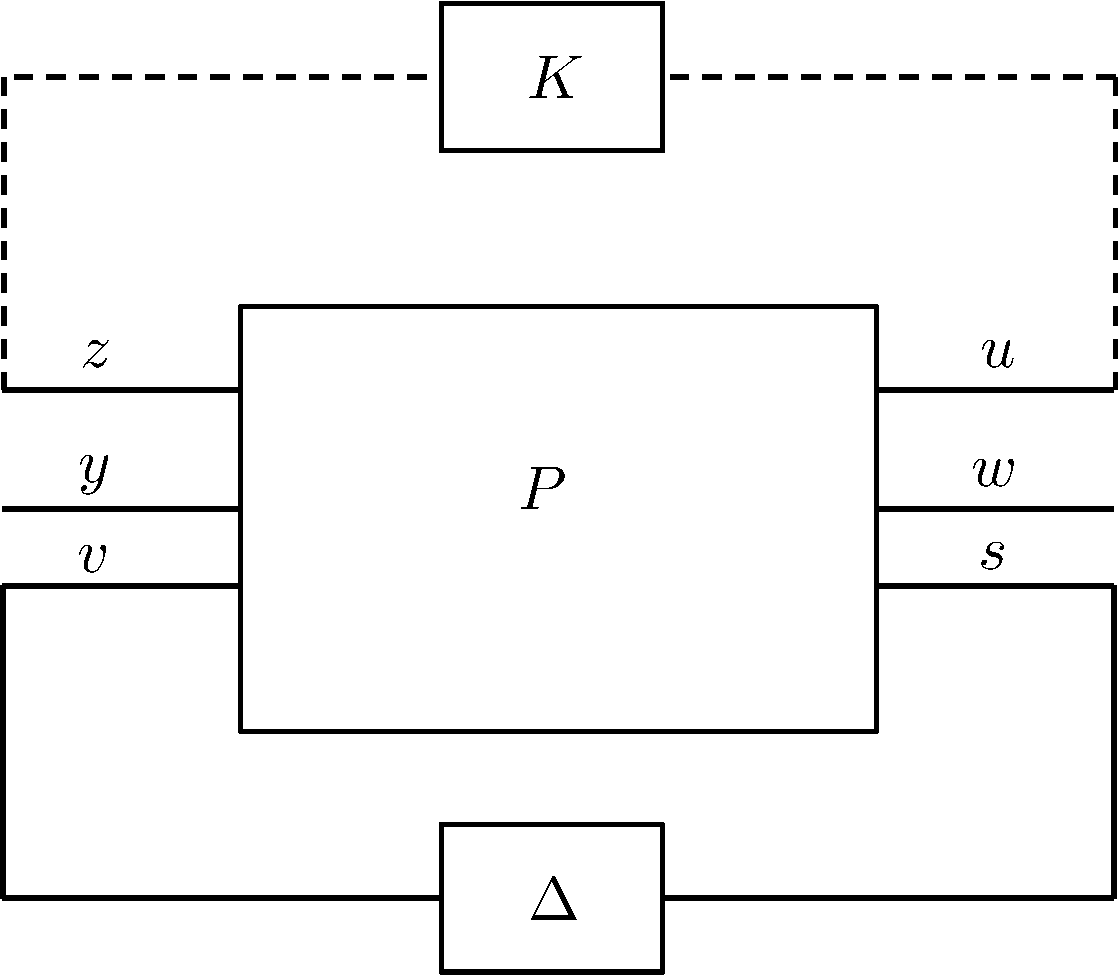
\includegraphics[width=.3\linewidth]{sys1.pdf}
\end{figure}


\section{Invalidation procedure}

For a particular $K$, given the $\mc K,P, \mc Q_{\Delta}, \mc Q_{W}$, given length $T$ observation
$(u_t, y_t, z_t)_{t=1}^{T}$, try to invalidate $K$.

Let's get a bit more concrete for the invalidation procedure and write it out here.

\section{Discussions}

Naive questions
\begin{enumerate}
\item how does this approach compare to controller synthesis with the IQC for $\Delta$? -- we can
  use the observation sequences without id + control.
\end{enumerate}


After studying the 0-th order question.
\begin{enumerate}
\item Start with a compact set for $\mc K$, we want to test one instance of $K$ and be able to rule
  out a measurable subset of $\mc K$.
\item Incorporate the information in the observation sequences to get a finer description of the
  uncertainty set $\Delta$ in terms of more IQCs in $\mc Q_{\Delta}$, which would give us more
  invalidation power.
\item Experiment design. Note that in the closed loop id, choosing a particular controller $K$
  determines the $u$ input sequence. We want to select a controller $K\in \mc K$ so that we can
  shave of a large portion of $\mc K$ with the invalidation procedure.
\end{enumerate}


\bibliographystyle{plain}
\bibliography{invalid}

\end{document}
